% !TEX root = ../dg.tex

\section{Distributions and Differential Ideals}
\label{sec:distributions and differential ideals}

\subsection{Linear Subspaces and Annihilators} 
\label{sub:linear_subspaces_and_annihilators}


So far, we've connected a geometric property of distributions (having integral manifolds) to an algebraic property in terms of vector fields tangent to the distribution (involutivity). Roughly speaking, we should expect algebraic properties of tangent vectors to carry over to algebraic properties of differential forms, so that's what we pursue next.

First, let's just focus on $\mathcal{D}(p) \subset T_p M$ for a particular point $p \in M$. This is just a subspace of a vector space. Of course, one way to describe a subspace is to describe the elements, for example by describing it as the span of a collection of vectors. Thinking dually, we could also describe the subspace in terms of the linear functionals which vanish on it.\footnote{Thought of another way, we can always think of a subspace as the kernel of some linear map. This is analogous to how in algebra we can think of normal subgroups as kernels of group homomorphisms.}

\begin{example}\label{ex:planes in R3}
	Think about the challenge of describing a 2-dimensional subspace $S \subset \R^3$. One way to do so is to give a basis for $S$; i.e., $S = \spa\{\vec{u},\vec{v}\}$ for some particular $\vec{u} , \vec{v} \in \R^3$. This is very convenient if we want to do computations involving vectors which we already know are in $S$; for example, if $ \vec{w} \in S$, then $\vec{w} = a \vec{u} + b \vec{v}$, and then for any linear transformation $T$ we know that $T(\vec{w}) = a T(\vec{u}) + b T(\vec{v})$, so we only really need to know $T(\vec{u})$ and $T(\vec{v})$ to describe what $T$ does to anything in $S$.
	
	On the other hand, this description is not so convenient if we don't already know $\vec{w}$ is in $S$. At the most basic level, we might be trying to determine whether some vector $\vec{w} \in \R^3$ is in $S$. We then have to determine whether the linear equation $a \vec{u} + b \vec{v} = \vec{w}$ has a solution. Admittedly, this is not a particularly challenging problem, but it might still be moderately annoying. 
	
	For this kind of problem, it is much nicer to describe $S$ in terms of linear functionals. For example, if we happen to know a vector $\vec{n}$ which is perpendicular to $S$ (for example, $\vec{n} = \vec{u} \times \vec{v}$, if we happen to have a basis $\{\vec{u}, \vec{v}\}$), then we could define the linear functional $\alpha \from \R^3 \to \R$ by $\alpha(\vec{w}) = \vec{n} \cdot \vec{w}$, and we see that $S = \ker \alpha$. Then it's easy to determine whether any given $\vec{w}$ is in $S$: just compute $\alpha(\vec{w})$ and see if it's zero. Of course, describing planes in $\R^3$ in terms of their (unit) normals is a very common and useful approach.
\end{example}

In \Cref{ex:planes in R3}, I used the fact that I had a preferred inner product on $\R^3$, but this isn't really necessary.

\begin{definition}\label{def:annihilator}
	Let $S$ be a subspace of a vector space $V$. The \emph{annihilator} of $S$, denoted $S^0$, is defined by
	\[
		S^0 := \{\phi \in V^\ast : \phi(v) = 0 \text{ for all } v \in S\}.
	\]
\end{definition}

The annihilator is a subset of the dual space $V^\ast$, and in fact it is easy to show it is a subspace:

\begin{proposition}\label{prop:annihilator is subspace}
	If $S$ is a subspace of a vector space $V$, then the annihilator $S^0$ is a subspace of $V^\ast$.
\end{proposition}

Moreover, as you might guess from the $\R^3$ example, $S$ and $S^0$ have complementary dimensions (here I'm assuming $\dim V$ is finite):
\[
	\dim S + \dim S^0 = \dim V.
\]
In fact, if $V$ has an inner product which we use to define an explicit isomorphism with $V^\ast$, then $S^0 \subset V^\ast$ will map to the orthogonal complement of $S$ under this isomorphism.

Annihilators also interact well with dual maps:

\begin{proposition}\label{prop:annihilators and duals}
	Suppose $V$ and $W$ are finite-dimensional vector spaces and $T \from V \to W$ is linear. Let $T^\ast \from W^\ast \to V^\ast$ be the corresponding dual map. Then
	\begin{enumerate}
		\item \label{it:prop annihilators ker} $\ker T^\ast = (\im T)^0$
		\item $\dim (\ker T^\ast) = \dim (\ker T) + \dim W - \dim V$
		\item $\im T^\ast = (\ker T)^0$
		\item $\dim(\im T^\ast) = \dim (\im T)$
	\end{enumerate}
\end{proposition}

For a proof, see \cite[\S 3.F]{axlerLinearAlgebraDone2015}.

Notice, in particular, that the choice of a basis $v_1, \dots , v_k$ for a subspace $S \subset V$ induces a linear map $B \from \R^k \to V$ defined by
\[
	B(e_i) = v_i,
\]
where $e_1, \dots , e_k$ is the standard basis for $\R^k$ (or really any basis). Of course, $S = \im(B)$, so \Cref{prop:annihilators and duals}\ref{it:prop annihilators ker} implies that
\[
	S^0 = (\im B)^0 = \ker B^\ast,
\]
where $B^\ast \from V^\ast \to \left(\R^k\right)^\ast$ is the dual map $B^\ast(\sigma)(v) = \sigma(B(v))$. So this gives a (semi-)explicit description of the linear functionals which vanish on $S$.

In the context of distributions on manifolds, $\mathcal{D}(p)$ is a subspace of $T_pM$, and the space of linear functionals $\left(T_pM\right)^\ast = \ext{1}\left(T_pM\right)^\ast$ is just the 1-forms on $M$ at $p$. So, more generally, we can talk about the differential forms on $M$ which vanish on $\mathcal{D}$. In fact, we've already seen this in \Cref{ex:standard contact structure}, where we described the standard contact structure on $\R^3$ as the kernel of a 1-form, namely $\ker(dz - p\, dx)$.

\subsection{Differential Ideals} 
\label{sub:differential_ideals}

Now we formalize our approach to describing distributions as kernels of differential forms.

\begin{definition}\label{def:annihilator ideal}
	Suppose $\mathcal{D}$ is a $d$-dimensional distribution on an $n$-dimensional manifold $M$ and define $\mathcal{I}(\mathcal{D}) \subset \Omega^\ast (M)$ to be the ring of differential forms which annihilate $\mathcal{D}$:
	\[
		\mathcal{I}(\mathcal{D}) := \bigcup_k \left\{ \omega \in \Omega^k(M) : \omega(X_1, \dots , X_k) = 0 \text{ for all } X_1, \dots , X_k \in \mathcal{D} \right\}.
	\]
\end{definition}

If $\omega_1, \omega_2 \in \mathcal{I}(\mathcal{D})$, then $\omega_1 + \omega_2 \in \mathcal{I}(\mathcal{D})$ and $\omega_1 \wedge \omega_2 \in \mathcal{I}(\mathcal{D})$, so this really is a ring.

In fact, if $\omega \in \mathcal{I}(\mathcal{D}) \cap \Omega^k(M)$ and $\eta \in \Omega^\ell(M)$, then
\[
	\omega \wedge \eta (X_1, \dots , X_{k+\ell}) = \sum_{\sigma \in S(k,\ell)} \sgn(\sigma) \omega(X_{\sigma(1)}, \dots , X_{\sigma(k)}) \eta(X_{\sigma(k+1)}, \dots , X_{\sigma(k+\ell)}) = 0,
\]
so $\omega \wedge \eta \in \mathcal{I}(\mathcal{D})$, which means that $\mathcal{I}(\mathcal{D})$ is actually an ideal, usually called either the \emph{annihilator ideal} of $\mathcal{D}$ or just the \emph{annihilator} of $\mathcal{D}$.

We've seen before in the proof of \Cref{thm:Frobenius} that any point $p \in M$ is contained in a coordinate chart $(U,\phi)$ with local coordinates $x_1, \dots , x_n$ so that $\mathcal{D}(p) = \spa \left\{\frac{\partial}{\partial x_1}, \dots , \frac{\partial}{\partial x_d} \right\}$. If $\xi_1, \dots , \xi_n$ are the dual 1-forms (i.e., $\xi_i = dx_i$), then $\xi_{d+1}, \dots , \xi_n$ are independent and generate $\mathcal{I}(\mathcal{D})$, which proves:

\begin{lemma}\label{lem:annihilator generators}
	For any $d$-dimensional distribution $\mathcal{D}$, the annihilator ideal $\mathcal{I}(\mathcal{D})$ is locally generated by $n-d$ independent $1$-forms $\xi_{d+1},\dots , \xi_n$.
\end{lemma}

On the other hand:

\begin{lemma}\label{lem:ideal gives distribution}
	If $\mathcal{I} \subset \Omega^\ast(M)$ is an ideal locally generated by $n-d$ independent $1$-forms, then there is a $d$-dimensional distribution $\mathcal{D}$ on $M$ so that $\mathcal{I} = \mathcal{I}(\mathcal{D})$.
\end{lemma}

\begin{proof}
	Let $\omega_{d+1}, \dots , \omega_n$ be the independent 1-forms generating $\mathcal{I}$ in a neighborhood of $p \in M$. Then define $\mathcal{D}(p) \subset T_pM$ to be the $d$-dimensional subspace annihilated by the linear functionals $\left(\omega_{d+1}\right)_p, \dots , \left(\omega_n\right)_p$. Then $\mathcal{D} = \bigcup_{p \in M} \mathcal{D}(p)$ is the desired distribution.
\end{proof}

Now we can give an alternative version of the Frobenius theorem in terms of annihilator ideals:

\begin{theorem}[Frobenius Theorem, version 2]\label{thm:Frobenius v2}
	A distribution $\mathcal{D}$ on $M$ is involutive (and hence integrable) if and only if $\mathcal{I}(\mathcal{D})$ is closed under taking exterior derivatives: $d(\mathcal{I}(\mathcal{D})) \subseteq \mathcal{I}(\mathcal{D})$.
\end{theorem}

\begin{definition}\label{def:differential ideal}
	An ideal $\mathcal{I} \subset \Omega^\ast(M)$ is called a \emph{differential ideal} if $d(\mathcal{I}) \subseteq \mathcal{I}$.
\end{definition}

So a restatement of \Cref{thm:Frobenius v2} is that a distribution is involutive if and only if its annihilator ideal is a differential ideal.

\begin{proof}[Proof of \Cref{thm:Frobenius v2}]
	Locally choose $\xi_1, \dots , \xi_n$ that span $\left(T_pM\right)^\ast = \ext{1}\left(\left(T_pM\right)^\ast\right)$ so that $\xi_{d+1}, \dots , \xi_n$ generate $\mathcal{I}(\mathcal{D})$ in a neighborhood of $p \in M$. Let $X_1, \dots , X_n$ be the dual vector fields so that $\xi_i(X_j) = \delta_{ij}$. Then $X_1, \dots , X_d$ span $\mathcal{D}$ and $\mathcal{D}$ is involutive if and only if $[X_i, X_j] \in \mathcal{D}$ for all $1 \leq i, j \leq d$.
	
	But now we get to use Cartan's Magic Formula (\Cref{thm:cartan}), which says that $\mathcal{L}_X \omega = \iota_X d\omega + d \iota_X \omega$. Then for any $1$-form $\omega$ and any $X,Y \in \mathfrak{X}(M)$, this implies that
	\begin{align*}
		d \omega(X,Y) = (\iota_X d\omega)(Y) & = (\mathcal{L}_X \omega)(Y)-(d \iota_X \omega)(Y) \\
		& = \mathcal{L}_X(\omega(Y))-\omega(\mathcal{L}_X(Y))-(d\omega(X))(Y) \\
		& = X(\omega(Y))-\omega([X,Y]) - Y(\omega(X)),
	\end{align*}
	since $\omega(X)$ and $\omega(Y)$ are functions.
	
	We record this as a lemma:
	
	\begin{lemma}\label{lem:d 1-form Cartan}
		Suppose $\omega \in \Omega^1(M)$ and $X,Y \in \mathfrak{X}(M)$. Then
		\[
			d \omega(X,Y) = X(\omega(Y))- Y(\omega(X))-\omega([X,Y]).
		\]
	\end{lemma}
	
	This implies that, if $1 \leq i, j \leq d$ and $d+1 \leq k \leq n$,
	\[
		d\xi_k(X_i,X_j) = X_i(\xi_x(X_j)) - X_j(\xi_k(X_i)) - \xi_k([X_i,X_j]) = X_i(0) - X_j(0) - \xi_k([X_i,X_j]) = - \xi_k([X_i,X_j]).
	\]
	This is zero for all such $i,j,k$ if and only if $\mathcal{D}$ is involutive. So $\mathcal{I}(\mathcal{D})$ is a differential ideal if and only if $\mathcal{D}$ is involutive.
\end{proof}

\begin{example}
	Recall yet again \Cref{sec:S^3 example} and our left-invariant vector fields $X,Y,Z$ and dual left-invariant 1-forms $\alpha, \beta, \gamma$ on $S^3$. Let $\zeta = \spa\{Y,Z\} = \ker \alpha$. Recall from \Cref{ex:S^3 standard contact structure} that $[Y,Z] = 2X \notin \zeta$, so $\zeta$ is not involutive, which by the original Frobenius Theorem (\Cref{thm:Frobenius}) implies that $\zeta$ is not integrable. We can also see this using \Cref{thm:Frobenius v2}: certainly $\alpha \in \mathcal{I}(\zeta)$, but as we saw in \Cref{ex:cartan and S^3},
	\[
		d\alpha = -2 \beta \wedge \gamma
	\]
	which is not in $\mathcal{I}(\zeta)$ since $-2\beta \wedge \gamma(Y,Z) = -2 \neq 0$, so $\mathcal{I}(\zeta)$ is not a differential ideal.
\end{example}

We (finally) have all the tools in place to start using this distribution machinery to prove \Cref{thm:Lie group Lie algebra correspondence}, which said that Lie algebra homomorphisms induce Lie group homomorphisms.

Here's an intermediate result:

\begin{theorem}\label{thm:identical Lie algebra homomorphisms imply identical Lie group homomorphisms}
	Let $G$ be a connected Lie group and let $f_1, f_2 \from G \to H$ be Lie group homomorphisms so that the Lie algebra homomorphisms $df_1, df_2 \from \mathfrak{g} \to \mathfrak{h}$ are identical. Then $f_1 \equiv f_2$.
\end{theorem}


Let's start trying to prove this and see where we run into trouble. Since $df_1 = df_2$ as maps $\mathfrak{g} \to \mathfrak{h}$, the dual maps $f_1^\ast = f_2^ \ast$ as maps $\mathfrak{h}^\ast \to \mathfrak{g}^\ast$, where we identify $\mathfrak{g}^\ast$ and $\mathfrak{h}^\ast$ with the left-invariant 1-forms on $G$ and $H$, respectively.\footnote{Notice that a Lie group homomorphism $f$ really does pull back left-invariant forms to left-invariant forms: for $\omega$ left-invariant on $H$ and $g \in G$,
\[
	L_g^\ast f^\ast \omega = (f \circ L_g)^\ast \omega = (L_{f(g)} \circ f)^\ast \omega = f^\ast L_{f(g)}^\ast \omega = f^\ast \omega,
\]
where the second equality follows by the same argument as in the proof of \Cref{prop:Lie group hom implies Lie alg hom}.}
	
Suppose $\omega_1 , \dots, \omega_n$ is a basis for the left-invariant forms on $H$. Then we know that $f_1^\ast \omega_i = f_2^\ast \omega_i$ for all $i = 1, \dots , n$, and the question is whether this is enough to show that $f_1 \equiv f_2$.
	
Think of this as a special case of a more general problem: 
\begin{problem}\label{prob:map with specified forms}
	Suppose we have manifolds $M$ and $N$ of dimensions $m$ and $n$, respectively, and we have a basis $\omega_1, \dots , \omega_n$ for the 1-forms on $N$, as well as a preferred collection $\alpha_1, \dots , \alpha_n$ of 1-forms on $M$. Is there a (preferably unique) map $f \from M \to N$ so that 
	\[
		f^\ast \omega_i = \alpha_i
	\]
	for all $i = 1, \dots , n$?
\end{problem}


\begin{example}
	Let $M = \R$, let $N = \R_{>0}$ be the positive reals, let $\omega = \frac{1}{y} \, dy \in \Omega^1(N)$, and let $\alpha = dx \in \Omega^1(M)$. If there is some $f \from M \to N$ so that $f^\ast \omega = \alpha$, then it must be the case that, for each $r \in \R$,
	\[
		1 = dx_r\left(\frac{\partial}{\partial x} \right) = \alpha_r\left(\frac{\partial}{\partial x} \right) = (f^\ast \omega)_r\left(\frac{\partial}{\partial x} \right) = \omega_{f(r)} \left(df_r\frac{\partial}{\partial x} \right) = \omega_{f(r)} \left((f\circ \gamma)'(0)\right),
	\]
	where $\gamma(0) = r$ and $\gamma'(0) = \frac{\partial}{\partial x}$; for example, $\gamma(t) = r+t$. In this case, $(f\circ \gamma)(t) = f(r+t)$, so $(f\circ \gamma)'(0) = f'(r) \frac{\partial}{\partial y}$, and hence we see that
	\[
		1 = \omega_{f(r)} \left((f\circ \gamma)'(0)\right) = \omega_{f(r)}\left( f'(r) \frac{\partial}{\partial y}\right) = \frac{1}{f(r)} dy \left( f'(r) \frac{\partial}{\partial y}\right) = \frac{1}{f(r)}f'(r).
	\]
	
	This can be solved, for example with $f_c(r) = c e^r$ for any positive constant $c > 0$. If we specify that $f(0) = 1$, then that fixes $c=1$ and we have the unique solution $f(r) = e^r$.
	
	To make this more geometric, for each $c > 0$ consider the graph of $f_c$, shown in \Cref{fig:exp graph}:
	\[
		\Gamma_c := \left\{ \left(r, f_c(r) \right) : r \in \R\right\} = \left\{ \left(r, ce^r \right) : r \in \R\right\}.
	\]
	\begin{figure}[htbp]
		\centering
			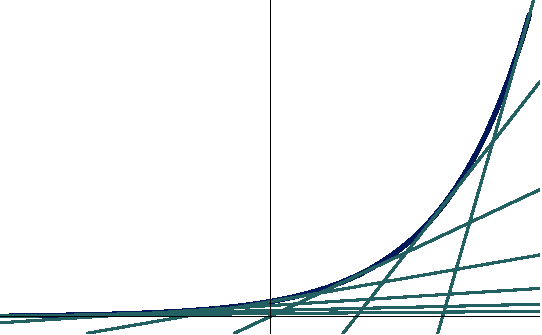
\includegraphics[height=1.3in]{expgraph}
		\caption{The graph of the function $f_c(r) = ce^r$, shown with its family of tangent lines.}
		\alttext{The graph of an exponential function, shown as a thick curve, together with a collection of its tangent lines, shown as thin lines.}
		\label{fig:exp graph}
	\end{figure}
	Notice that the tangent line to a point $(r, ce^r) \in \Gamma_c$ is spanned by the vector $(1,ce^r) = \frac{\partial}{\partial x} + c e^r \frac{\partial}{\partial y}$. If we write $(r, ce^r)$ as $(x,y)$, then this vector is just $\frac{\partial}{\partial x} + y \frac{\partial}{\partial y}$, which defines a non-vanishing vector field (and hence a line field or 1-dimensional distribution) on all of the upper half-plane $\R \times \R_{>0}$. And for each $c$ the graph $\Gamma_c$ is an integral manifold of this distribution. See \Cref{fig:exp line field}.
	\begin{figure}[htbp]
		\centering
			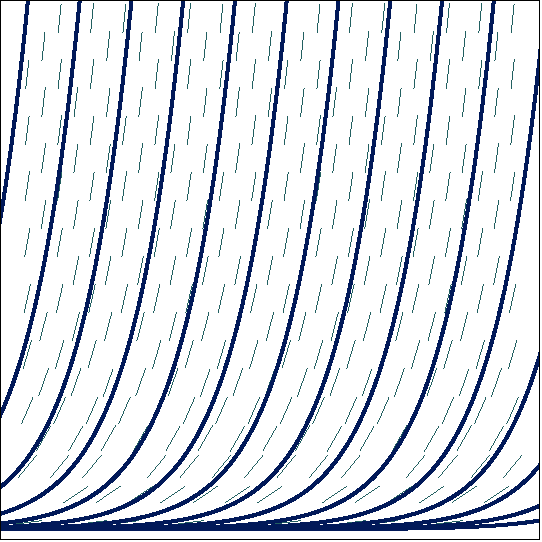
\includegraphics[height=2in]{expgraphfield}
		\caption{The integral manifolds of the line field $\frac{\partial}{\partial x} + y \frac{\partial}{\partial y}$ on the upper half-plane.}
		\alttext{Graphs of exponential functions, shown as thick curves, on a background of the line field described in the caption, depicted by thin line segments at various points.}
		\label{fig:exp line field}
	\end{figure}
	
	Finally, we see that the annihilator ideal of this distribution is generated by the 1-form dual to $\frac{\partial}{\partial x} + y \frac{\partial}{\partial y}$, namely $\mu = dx - \frac{1}{y} \, dy$. But now this is a form we could have constructed on $M \times N = \R \times \R_{>0}$ without knowing anything at all about $f$: if $\pi_1$ and $\pi_2$ are the obvious projections onto the first and second factors, then $\mu = \pi_1^\ast \alpha - \pi_2^\ast \omega$.
\end{example}

For arbitrary $M$ and $N$ with $\alpha_i$ and $\omega_i$ given as above, define $\mu_i \in \Omega^1(M \times N)$ by 
\[
	\mu_i := \pi_1^\ast \alpha_i - \pi_2^\ast \omega_i
\]
and let $\mathcal{I}$ be the ideal generated by the $\mu_i$. 

This gives a strategy for solving \Cref{prob:map with specified forms}: suppose there were a map satisfying our condition $f^\ast \omega_i = \alpha_i$ for all $i$, and let $\Gamma \from M \to M \times N$ be the graph of $f$: $\Gamma(x) = (x,f(x))$ for all $x \in M$. Then I claim that $\Gamma$ is an integral manifold of $\mathcal{I}$ (really, of the distribution $\mathcal{D}$ so that $\mathcal{I} = \mathcal{I}(\mathcal{D})$).

To see this, it suffices to show that $\Gamma^\ast \mu_i = 0$ for all $i$. Since $\pi_1 \circ \Gamma = \operatorname{id}_M$ and $\pi_2 \circ \Gamma = f$,
\[
	\Gamma^\ast \mu_i = \Gamma^\ast(\pi_1^\ast \alpha_i - \pi_2^\ast \omega_i) = \Gamma^\ast(\pi_1^\ast f^\ast \omega_i - \pi_2^\ast \omega_i)  = (\pi_1 \circ \Gamma)^\ast f^\ast \omega_i - (\pi_2 \circ \Gamma)^\ast \omega_i = f^\ast \omega_i - f^\ast \omega_i = 0.
\]
So this says that if $f$ exists, its graph is an integral manifold of the ideal $\mathcal{I}$, which of course means that $\mathcal{I}$ must be a differential ideal (by \Cref{thm:Frobenius v2}). In other words, $\mathcal{I}$  being a differential ideal is a necessary condition for such an $f$ to exist.